\documentclass[a4paper]{llncs}
\usepackage{amsmath}
\usepackage{tikz}
\usetikzlibrary{calc,shapes.geometric}
\usetikzlibrary{shapes}
\usetikzlibrary{automata,positioning,decorations.pathreplacing}

\begin{document}

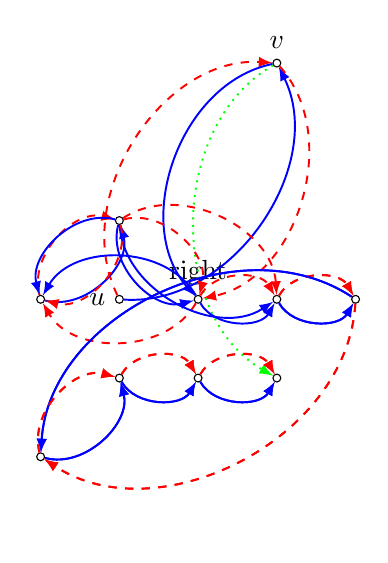
\begin{tikzpicture}[every state/.style={inner sep=0pt,minimum size=1mm}]
\node[state,label={above:$v$}] (V) at (0,0){};
\node[state,label={left:$u$}] (U) at (-2,-3){};
\node[state,label={right}](C) at (-1,-3){};
\node[state] (B) at (-3,-3){};
\node[state] (A) at (-2,-2){};
\node[state] (D) at (0,-3){};
\node[state] (E) at (1,-3){};
\node[state] (F) at (-3,-5){};
\node[state] (G) at (-2,-4){};
\node[state] (H) at (-1,-4){};
\node[state] (I) at (0,-4){};

\draw[-latex,color=red,dashed,line width=0.7pt] (U) to[bend left=60] (V);
\draw[-latex,color=blue,solid,line width=0.7pt] (U) to[bend right=60] (V);

\draw[-latex,color=red,dashed,line width=0.7pt] (V) to[bend left=60] (C);
\draw[-latex,color=blue,solid,line width=0.7pt] (V) to[bend right=60] (C);

\draw[-latex,color=red,dashed,line width=0.7pt] (C) to[bend left=60] (B);
\draw[-latex,color=blue,solid,line width=0.7pt] (C) to[bend right=60] (B);

\draw[-latex,color=red,dashed,line width=0.7pt] (B) to[bend left=60] (A);
\draw[-latex,color=blue,solid,line width=0.7pt] (B) to[bend right=60] (A);

\draw[-latex,color=red,dashed,line width=0.7pt] (A) to[bend left=60] (D);
\draw[-latex,color=blue,solid,line width=0.7pt] (A) to[bend right=60] (D);

\draw[-latex,color=red,dashed,line width=0.7pt] (D) to[bend left=60] (E);
\draw[-latex,color=blue,solid,line width=0.7pt] (D) to[bend right=60] (E);

\draw[-latex,color=red,dashed,line width=0.7pt] (E) to[bend left=60] (F);
\draw[-latex,color=blue,solid,line width=0.7pt] (E) to[bend right=60] (F);

\draw[-latex,color=red,dashed,line width=0.7pt] (F) to[bend left=60] (G);
\draw[-latex,color=blue,solid,line width=0.7pt] (F) to[bend right=60] (G);

\draw[-latex,color=red,dashed,line width=0.7pt] (G) to[bend left=60] (H);
\draw[-latex,color=blue,solid,line width=0.7pt] (G) to[bend right=60] (H);

\draw[-latex,color=red,dashed,line width=0.7pt] (H) to[bend left=60] (I);
\draw[-latex,color=blue,solid,line width=0.7pt] (H) to[bend right=60] (I);

\draw[-latex,color=green,dotted,line width=0.7pt] (V) to[bend right=60] (I);

\draw[-latex,color=blue,solid,line width=0.7pt] (A) to[bend right=60] (B);
\draw[-latex,color=red,dashed,line width=0.7pt] (A) to[bend left=60] (B);

\draw[-latex,color=blue,solid,line width=0.7pt] (A) to[bend right=60] (C);
\draw[-latex,color=red,dashed,line width=0.7pt] (A) to[bend left=60] (C);

\draw[-latex,color=blue,solid,line width=0.7pt] (C) to[bend right=60] (D);
\draw[-latex,color=red,dashed,line width=0.7pt] (C) to[bend left=60] (D);

\draw[-latex,color=blue,solid,line width=0.7pt] (D) to[bend right=60] (E);
\draw[-latex,color=red,dashed,line width=0.7pt] (D) to[bend left=60] (E);

\draw[-latex,color=blue,solid,line width=0.7pt] (E) to[bend right=60] (F);
\draw[-latex,color=red,dashed,line width=0.7pt] (E) to[bend left=60] (F);

\draw[-latex,color=blue,solid,line width=0.7pt] (F) to[bend right=60] (G);
\draw[-latex,color=red,dashed,line width=0.7pt] (F) to[bend left=60] (G);

\draw[-latex,color=blue,solid,line width=0.7pt] (G) to[bend right=60] (H);
\draw[-latex,color=red,dashed,line width=0.7pt] (G) to[bend left=60] (H);

\draw[-latex,color=blue,solid,line width=0.7pt] (H) to[bend right=60] (I);
\draw[-latex,color=red,dashed,line width=0.7pt] (H) to[bend left=60] (I);
\end{tikzpicture}

\end{document}